\documentclass[titlepage]{book}
\usepackage[]{graphicx}\usepackage[]{color}
% maxwidth is the original width if it is less than linewidth
% otherwise use linewidth (to make sure the graphics do not exceed the margin)
\makeatletter
\def\maxwidth{ %
  \ifdim\Gin@nat@width>\linewidth
    \linewidth
  \else
    \Gin@nat@width
  \fi
}
\makeatother

\definecolor{fgcolor}{rgb}{0.345, 0.345, 0.345}
\newcommand{\hlnum}[1]{\textcolor[rgb]{0.686,0.059,0.569}{#1}}%
\newcommand{\hlstr}[1]{\textcolor[rgb]{0.192,0.494,0.8}{#1}}%
\newcommand{\hlcom}[1]{\textcolor[rgb]{0.678,0.584,0.686}{\textit{#1}}}%
\newcommand{\hlopt}[1]{\textcolor[rgb]{0,0,0}{#1}}%
\newcommand{\hlstd}[1]{\textcolor[rgb]{0.345,0.345,0.345}{#1}}%
\newcommand{\hlkwa}[1]{\textcolor[rgb]{0.161,0.373,0.58}{\textbf{#1}}}%
\newcommand{\hlkwb}[1]{\textcolor[rgb]{0.69,0.353,0.396}{#1}}%
\newcommand{\hlkwc}[1]{\textcolor[rgb]{0.333,0.667,0.333}{#1}}%
\newcommand{\hlkwd}[1]{\textcolor[rgb]{0.737,0.353,0.396}{\textbf{#1}}}%
\let\hlipl\hlkwb

\usepackage{framed}
\makeatletter
\newenvironment{kframe}{%
 \def\at@end@of@kframe{}%
 \ifinner\ifhmode%
  \def\at@end@of@kframe{\end{minipage}}%
  \begin{minipage}{\columnwidth}%
 \fi\fi%
 \def\FrameCommand##1{\hskip\@totalleftmargin \hskip-\fboxsep
 \colorbox{shadecolor}{##1}\hskip-\fboxsep
     % There is no \\@totalrightmargin, so:
     \hskip-\linewidth \hskip-\@totalleftmargin \hskip\columnwidth}%
 \MakeFramed {\advance\hsize-\width
   \@totalleftmargin\z@ \linewidth\hsize
   \@setminipage}}%
 {\par\unskip\endMakeFramed%
 \at@end@of@kframe}
\makeatother

\definecolor{shadecolor}{rgb}{.97, .97, .97}
\definecolor{messagecolor}{rgb}{0, 0, 0}
\definecolor{warningcolor}{rgb}{1, 0, 1}
\definecolor{errorcolor}{rgb}{1, 0, 0}
\newenvironment{knitrout}{}{} % an empty environment to be redefined in TeX

\usepackage{alltt}
\newcommand{\SweaveOpts}[1]{}  % do not interfere with LaTeX
\newcommand{\SweaveInput}[1]{} % because they are not real TeX commands
\newcommand{\Sexpr}[1]{}       % will only be parsed by R


\usepackage{bwstyle}

\title{\huge \textbf{ R- a tool for statistical analysis }\vspace{+1cm}  }
\subtitle{A modern introduction using tidyverse}
\author{{\LARGE \emph{Brian Williams}}\vspace{+1cm} \\
 Epidemiology and Global Health Unit,\\
 Department of Public Health and Medicine,\\
 Umeå University \vspace{+8cm}}
 

\date{\today}



\begin{document}
\begin{knitrout}
\definecolor{shadecolor}{rgb}{0.969, 0.969, 0.969}\color{fgcolor}\begin{kframe}
\begin{alltt}
\hlkwd{library}\hlstd{(knitr)}
\hlkwd{set_parent}\hlstd{(}\hlstr{"../tidyRcourseBook.rnw"}\hlstd{)}
\hlkwd{library}\hlstd{(tidyverse)}
\end{alltt}


{\ttfamily\noindent\itshape\color{messagecolor}{\#\# -- Attaching packages ------------------------------------------------------------------------------------------------------------- tidyverse 1.3.0 --}}

{\ttfamily\noindent\itshape\color{messagecolor}{\#\# v ggplot2 3.2.1\ \ \ \  v purrr\ \  0.3.3\\\#\# v tibble\ \ 2.1.3\ \ \ \  v dplyr\ \  0.8.3\\\#\# v tidyr\ \  1.0.2\ \ \ \  v stringr 1.4.0\\\#\# v readr\ \  1.3.1\ \ \ \  v forcats 0.4.0}}

{\ttfamily\noindent\itshape\color{messagecolor}{\#\# -- Conflicts ---------------------------------------------------------------------------------------------------------------- tidyverse\_conflicts() --\\\#\# x dplyr::filter() masks stats::filter()\\\#\# x dplyr::lag()\ \ \ \ masks stats::lag()}}\begin{alltt}
\hlstd{warn} \hlkwb{<-} \hlnum{FALSE}
\hlstd{EVAL} \hlkwb{<-} \hlnum{TRUE}
\end{alltt}
\end{kframe}
\end{knitrout}



\chapter{Lecture 1 - Introduction to R and RStudio }\label{L1}
\section*{- and a glimpse of what's coming!}

\author{Brian Williams $<$\href{mailto:bjw649@gmail.com}%
{bjw649@gmail.com}$>$}

\section{Summary}
In this session there will be a brief introduction to RStudio and reading, manipulating, cross-tabulating and visualizing data from dataframes using the \emph{tidyverse} package in RStudio.

\textbf{Note:} In this lecture some advanced features of R will be demonstrated. \textbf{Don't worry about what appears to be complex commands}. You will be shown how to easily step through the code and see what comes from it! 

RStudio is the most widely used integrated development environment (IDE) for R and provides excellent support for documenting code for reproducibility.

\subsection{Tidyverse}
Tidyverse is a suite of modern R software, largely developed by Hadley Wickham and colleagues at RStudio, which aims to reduce R's learning curve by providing a more consistent way of dealing with dataframes. 

Not all the software in tidyverse is limited to dataframes, but that is its broad goal.   Tidyverse is still under development, though what we will use is well tried and tested. 

There are still many procedures of interest to us in 'Core' R, which currently lie outside tidyverse and we will use these as the need arises. 

Check out the freely available \href{https://r4ds.had.co.nz/index.html}{web version of the book} "R for data science" by Hadley and Garret Grolemund \cite{Wickham2016}. This course is inspired by the approach in that book.  Much of the material in this course is extracted and simplified from an earlier course aimed at research students in the Medical Faculty. The earlier course notes are available in the resources folder (R4researchFeb2016.pdf) and may provide expanded background on many topics. The R4researchFeb2016.pdf notes are also live-indexed and have a live table of contents, so you should be able to find things in those notes reasonably easily.

\section{Preliminaries}

Load and install R, RStudio and extract the folders from R\_Course.zip (available on the Course pages on Cambro) in a convenient folder on your computer. (Extracting will normally create a new folder called R\_Course).

\section{Getting started}

\textbf{Note that you will follow the steps in this section at the beginning of every Lecture and Tutorial.}

Assuming you have taken all the steps in the Preliminaries section:

Navigate to your R\_Course folder. It should contain 3 folders, Data, myCode, Resources and files called ReadMe.pdf, Preliminaries.pdf and RCourseOutlineRev2019.pdf. 

\textbf{Open} R\_Notes.pdf, located in your Resources folder.

You will need to open the Resources folder and then the R\_Notes.pdf at the beginning of each class. You will be able to follow the class presentation and use the live links in the notes for each Lecture and Tutorial. Note that the index is also live-linked so you should be able to find your way about without too much trouble. (If you are using Acrobat and Windows, [Alt <-] pressed together will take you back from the index to where you clicked on the index link.)

Now: 

\begin{enumerate}

\item {\textbf{Open RStudio}, by clicking on the icon.}

\item{From the File menu in RStudio, \textbf{open the folder courseCode} in the folder R\_Course/Resources  (Select [File -> Open File...].) In these notes, menu items will be indicated in square brackets with arrows as shown in the previous sentence.  The folder \texttt{courseCode} contains all of the R code used in the notes.  Each Lecture and Tutorial is clearly identified.} 

\item{Double click on Lecture1.R and it will open in The Edit Pane  of your RStudio window (see Figure~\ref{fig:Screenshot}).}

\item{Use [File -> Save As...] in the file menu to save the file in your myRcode folder.}  

\item{Use mouse/menu to \textbf{set the working directory}\index{RStudio!setting working directory} to the file location: [Session -> Set Working Directory -> To Source File Location]. You will see in the Console Pane (bottom left of the screen, see Figure~\ref{fig:Screenshot}) that the R function for this is \texttt{setwd()}\index{Core functions!setwd()}.}

\end{enumerate}

\begin{figure}[!ht]
\graphicspath{{./Images/}}
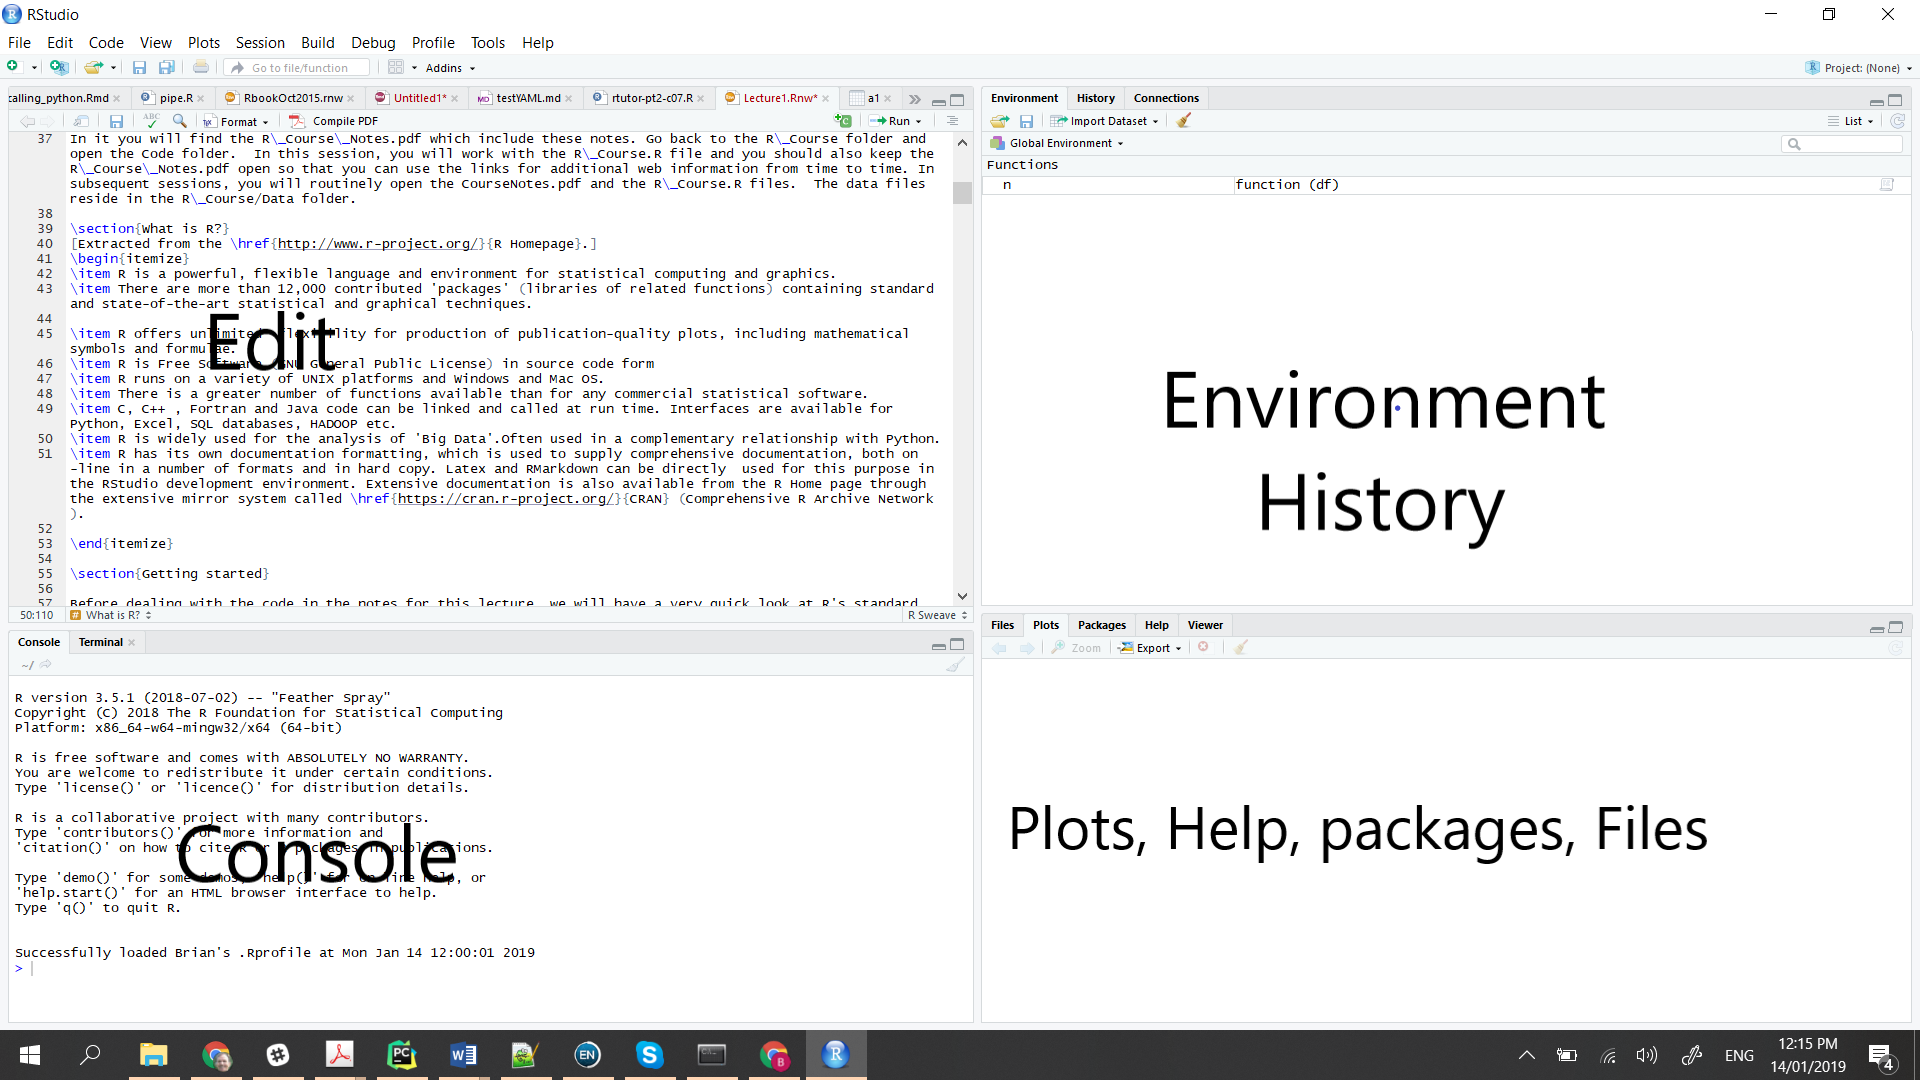
\includegraphics[width = 16cm, height = 8cm]{Screenshot1.png}
\caption{The four panes in the RStudio window}
\label{fig:Screenshot}
\end{figure}

This sets your working directory to the myCode folder. \textbf{This is an important step!}  Without it, R won't be able to find the data files, which have all been put in the Data folder which is found relative to the location of your myCode folder. Both the Data folder and your myCode folder are in the R\_Course folder (their 'parent' folder). If you are not clear take a look at Section~\ref{DataStructure} in the Appendix.

You will see that the top left window pane of the RStudio interface now contains the Lecture1.R file.   We refer  to this pane as the \textbf{Edit pane}\index{RStudio!Edit pane} or 'script' pane or window (See Figure~\ref{fig:Screenshot}.  Notice that the name of the file is shown on a 'tab' above the window. You can use this pane to edit a number of different scripts using the tabs, and from this pane you can run selected code directly, by clicking on the 'Run' button on the pane's toolbar.

If you compare the text in beige, below in these notes, with the first 'block' in the Edit pane, you will see that in the notes, each line is preceded by '\#\#'. This is just a decoration generated by the software for these notes. The proper R statements without '\#\#' are in your Lecture1.R file, as displayed in the edit pane of RStudio.

Beneath the Edit pane, is the \textbf{Console pane}\index{RStudio!Console Pane}(See Figure~\ref{fig:Screenshot}), in which the evaluated R commands will appear. It has a '>' symbol as a prompt, which indicates that the Console Pane is ready for your next command.  You can also paste commands into this pane for execution, or edit a previous command using the up-arrow to retrieve it. 

If you see a '+' prompt, it is an indication that you have entered an incomplete command and R is waiting for the rest of the command. If you can see what you have left out, enter it and press return and the command will be executed.  Sometimes it will not be clear what is missing and you may have to start again -  in that situation to return to the '>' prompt you must press the 'Escape' key.  

To clear everything in the console window, press 'Ctrl+L'.

The top right pane (see Figure~\ref{fig:Screenshot}) is the \textbf{Environment/History pane}\index{RStudio!Environment/History pane} (selectable using the tabs). The environment will contain basic information about variables which the user has introduced. There are two groups. At the top is 'Data' which consists of two-dimensional arrays (dataframes look like a spreadsheet table) and underneath are 'Variables' which are all other data objects defined by the user in the session.

The history tab contains the sequence of R commands which the user has entered during the session (and earlier). You can execute these directly by selecting them with a mouse click and then clicking on the tool above, labelled 'To Console'. If you want to insert these commands in your edit window, click where you wanted the commands inserted and then click on the 'To Source ' button in the History Pane.


The bottom right pane has a variety of displays (Files, Plots, Packages and Help) indicated and accessed by the tabs.

Now before we begin -

The text in the sections of the notes in the coloured (beige?) boxes between the dashed lines:

\# - - - - - - - - - - - - - - - - - - - - - - - - - - - - - - - - - - - - - - - - -

are sequences of R commands (scripts). You will find an extraction of all these scripts in Lecture1.R, Tutorial2.R etc in the Resources/Course\_R\_Code folder.
Scripts may include comments. Lines preceded with the \# symbol (like the dashed line above) may be used to explain to a reader what the script is doing - or (as here) provide a way of separating or identifying lines of text. These lines preceded with the \# symbol are ignored by R's interpretation (computation) of the script.

You can run the example scripts in Lecture1.R in three ways.
(The easiest way is the last one!)

First: \textbf{select} (highlight) the code using your mouse.

Then \textbf{copy} (using the Windows shortcut, \texttt{Ctrl-c)}. (\texttt{Command-c on a Mac})

Now \textbf{click} in the Console window of RStudio (the window below), and \textbf{paste} the code (\texttt{Ctrl-v}). (Mac: \texttt{Command-v})

If nothing happens, in the console, press the return/enter key.

\textbf{Second:}, after highlighting the code, \textbf{click} on the 'Run' button\index{RStudio!Run button} near the top right of the Edit window.

\textbf{Third (best):} Place the cursor on the first line and press \texttt{Ctrl-enter}. The code in that line will execute and the cursor will move down to the next line of code. Repeat pressing \texttt{Ctrl-enter} until you have stepped through as much of the code as you want to execute.

Try these three methods with the following 4 lines of script:

\begin{knitrout}
\definecolor{shadecolor}{rgb}{0.969, 0.969, 0.969}\color{fgcolor}\begin{kframe}
\begin{alltt}
  \hlcom{##Normally distributed N(0,1) variates, mean, var}
  \hlcom{#-----------------------------------------------------------------------------------}
\hlkwd{set.seed}\hlstd{(}\hlnum{1121}\hlstd{)}  \hlcom{# set a seed for pseudo-random number generation}
\hlstd{(x} \hlkwb{<-} \hlkwd{rnorm}\hlstd{(}\hlnum{20}\hlstd{))}   \hlcom{# creates a vector, x, containing 20 N(0,1) variates}
\end{alltt}
\begin{verbatim}
##  [1]  0.1449583  0.4383221  0.1531912  1.0849426  1.9995449 -0.8118832
##  [7]  0.1602680  0.5858923  0.3600880 -0.0253084  0.1508809  0.1100824
## [13]  1.3596812 -0.3269946 -0.7163819  1.8097690  0.5084011 -0.5274603
## [19]  0.1327188 -0.1559430
\end{verbatim}
\begin{alltt}
\hlkwd{mean}\hlstd{(x)}         \hlcom{# computes the mean of the sample}
\end{alltt}
\begin{verbatim}
## [1] 0.3217385
\end{verbatim}
\begin{alltt}
\hlkwd{var}\hlstd{(x)}          \hlcom{# computes the variance of the sample}
\end{alltt}
\begin{verbatim}
## [1] 0.5714534
\end{verbatim}
\begin{alltt}
\hlcom{#----------------------------------------------------------------------------------}
\end{alltt}
\end{kframe}
\end{knitrout}

  Now \textbf{CLICK in the edit window} away from the selection to deselect (remove the highlight)!!!!

  If you don't, the highlighted code will be \textbf{LOST} as it is replaced by your next typed characters in the edit window.

It's easy to make this mistake (I do it frequently!) but if you realise you have done it, the edit menu provides an 'undo' item which will get the lost characters back for you. (\texttt{Ctrl Z} also works - and you can undo\index{RStudio!undo} several actions by pressing \texttt{Ctrl z} repeatedly). As with all kinds of editing on computers, it's a good idea to save your edited file using (\texttt{Ctrl S}) frequently. You can save \textbf{all} the files you have opened in RStudio, using (\texttt{Ctrl Alt S}).

\section{HELP!!}
There are various ways of getting help in R.
\begin{itemize}
\item{\texttt{??graph} searches the documentation for the word 'graph' and lists findings in the Help window (bottom right).}
\item{\texttt{?plot} is used to find help for a \emph{function} (the function \texttt{plot}, in this case). }
\item{Similarly, \texttt{help(fn)}\index{Core functions!help()} finds the documentation associated with the function named \texttt{fn}. It acts exactly the same as the previous one (the question mark form).}

\item{\texttt{example(fn)}\index{Core functions!example()}  prints a number of examples of the use of the function in the Console window.}
\item{Some packages have an introductory document called a 'vignette' which can be accessed with the function \texttt{vignette()}\index{Core functions!vignette()}, but you should start with \texttt{browseVignettes()}!}
\item{Try: \texttt{vignette('lmtest-intro')}.}
\item{\texttt{data()}\index{Core functions!data()} lists available data sets (and is used to load datasets, too).}
\end{itemize}

For more complex problems go to the Help window (click on the Help tab if it is not currently selected) and click on the Home icon (the picture of a little house in the tool bar of this window) and you will see links  to some of the various documentation on the CRAN web site.
Otherwise on the CRAN website itself you can look at \href{http://cran.r-project.org/doc/contrib/Torfs+Brauer-Short-R-Intro.pdf}{reference material} on the CRAN site.

.......or simply \emph{use Google} (often the best way for more complicated queries) If your problem is a little complicated, Google is likely to find something on the 'stackoverflow' site.  Take your time looking at material on this site.  Because there is a significant level of control on posting, the responses are more reliable than many other sites on the web. Look for a big green 'tick' for the best solution to a questioner's problem.

\section{Functions}
We have already used some \textbf{functions}\index{Functions!using} in R.  Functions are fundamental to the use of commands. Commands always use functions, though it may not always be apparent.

\begin{itemize}
\item{Functions appear as a character string followed by parenthesis (curved brackets) containing zero or more items called \textbf{arguments} separated by commas. These argument control the way the function behaves.}

\item{Most functions have multiple  arguments, which have been given \textbf{default values}. If you don't specify an argument when you 'call' (i.e. use) the function, its default value will be used.}

\item{We can change the defaults by specifying values for the arguments when we call the function. Arguments in all functions can be changed in this way but must conform to the requirements of the function, which may require, for example, that an argument be of a particular type, or that its length match that of another argument.}

\end{itemize}

To see how a function (say) \texttt{mean()}\index{Core functions!mean()} is used, enter \texttt{help(mean)} in the Console window and look at the output in the Help pane to the right. Help for functions can also be accessed by typing e.g. \texttt{?mean} in the Console window. Try it with \texttt{?sd}

There are other examples of functions in the \href{https://cran.r-project.org/doc/manuals/r-release/R-intro.html#Simple-examples}{on-line Manual} "An introduction to R" on the CRAN website. 

\section{Data frames: reading data and investigating them}\index{Core functions!data()}

In this section we'll see the power of R, but we won't try to look in detail at the function useage - that'll come later, so don't worry too much about the syntax of the commands (functions).

There are a number of functions which allow reading of data sets from other statistical software like SAS and Stata (see the package 'foreign'), but for the moment we'll deal with reading our data from a .csv file, perhaps created by spreadsheet software.\index{Data frame!reading from .csv} We are going to focus our efforts on a single R package called tidyverse, which you will see is implemented by calling the \texttt{library} function with tidyverse as its argument.  Before doing so, however, we need to install the package.

\subsection{Installing packages} 

Tidyverse contains a suite of modern R packages, mostly authored by Hadley Wickham and his colleagues at RStudio. Tidyverse focuses on the preparation, analysis and vizualization of dataframes - and that is the focus of this course.  

\subsubsection{Installing tidyverse}
Installing a package is easy. Go to [Tools->Install packages ...]. Type the name of the package (tidyverse) (it should be predicted) and then click on install. You will see some activity in the console window and then a message indicating that the installation is successful, followed by the Console Pane's standard prompt '>'.

When that's all done, go to the packages pane and click on the 'Packages' tab at the top. Use the window slider at the side or the search at the top to find the tidyverse package in the list. Click in the box on the left and you will see that the library command has been used in the Console window of RStudio. [The libary command will also include the directory path of all your installed packages.] Click on the blue name tidyverse and you will be taken to the help page for the package. All packages will have some kind of help file like this. The Description file may be a bit too terse, but if you click on the User guides..... link, you will usually find more digestible infomation.

\subsection{Reading a dataframe using the tidyverse package \texttt{readr}}

In \texttt{tidyverse}, the standard function for reading a .csv file is \texttt(read\_csv).

\begin{knitrout}
\definecolor{shadecolor}{rgb}{0.969, 0.969, 0.969}\color{fgcolor}\begin{kframe}
\begin{alltt}
  \hlcom{##Reading and summarising data frames}
  \hlcom{#----------------------------------------------------------------------------------}
\hlkwd{library}\hlstd{(tidyverse)}
\hlstd{bP}        \hlkwb{<-} \hlkwd{read_csv}\hlstd{(}\hlkwc{file}\hlstd{=}\hlstr{"../Data/BackPain.csv"}\hlstd{,} \hlkwc{na} \hlstd{=} \hlkwd{c}\hlstd{(}\hlstr{""}\hlstd{,}\hlstr{" "}\hlstd{,}\hlstr{"NA"}\hlstd{))}      \hlcom{# (1), (2), (3), (4)}
\end{alltt}


{\ttfamily\noindent\itshape\color{messagecolor}{\#\# Parsed with column specification:\\\#\# cols(\\\#\#\ \  .default = col\_character(),\\\#\#\ \  age = col\_double(),\\\#\#\ \  bmi = col\_double(),\\\#\#\ \  waistc = col\_double(),\\\#\#\ \  comorb = col\_double(),\\\#\#\ \  disability = col\_double(),\\\#\#\ \  height = col\_double()\\\#\# )}}

{\ttfamily\noindent\itshape\color{messagecolor}{\#\# See spec(...) for full column specifications.}}\begin{alltt}
\hlkwd{glimpse}\hlstd{(bP)}
\end{alltt}
\begin{verbatim}
## Observations: 34,122
## Variables: 24
## $ residence  <chr> "Urban", "Urban", "Urban", "Rural", "Rural", "Urban", "R...
## $ sex        <chr> "Female", "Female", "Female", "Male", "Female", "Female"...
## $ age        <dbl> 66, 63, 76, 64, 67, 74, 51, 80, 67, 75, 70, 68, 78, 55, ...
## $ wealthQ    <chr> "Q3", "Q4", "Q5 richest", "Q4", "Q1 poorest", "Q4", "Q3"...
## $ physical   <chr> "high phys act", "mod phys act", "high phys act", "high ...
## $ country    <chr> "China", "China", "China", "Mexico", "China", "China", "...
## $ backPain30 <chr> "No", "No", "No", "No", "No", "No", "No", "No", "No", "N...
## $ agegr      <chr> "60-69", "60-69", "70-79", "60-69", "60-69", "70-79", "5...
## $ maritalS   <chr> "Div/Wid/Sep", "Div/Wid/Sep", "Div/Wid/Sep", "Married/Co...
## $ eduS       <chr> "Compl Sec/HS", "Compl Sec/HS", "No primary", "Compl Pri...
## $ workS      <chr> "currently not working", "currently not working", "curre...
## $ bmi        <dbl> 23.87512, 19.43697, 28.56648, 26.06168, 26.97505, 21.504...
## $ bmi4       <chr> "Normal", "Normal", "Pre-Obese", "Pre-Obese", "Pre-Obese...
## $ waistc     <dbl> 92.0, 66.0, 85.0, 99.5, 90.2, 75.0, 96.0, 100.0, 94.3, N...
## $ smoke      <chr> "Never/Not Daily/Current", "Never/Not Daily/Current", "N...
## $ alcohol    <chr> "Abstainers", "Abstainers", "Abstainers", "Abstainers", ...
## $ arthritis  <chr> "no", "no", "no", "no", "no", "yes", "yes", "no", "yes",...
## $ angina     <chr> NA, "no", NA, "no", NA, "no", "no", "no", "no", NA, "no"...
## $ depression <chr> "no", "no", "no", "no", "no", "no", "no", "no", "no", "n...
## $ asthma     <chr> "no", "no", "no", "no", "no", "no", "no", "no", "no", "n...
## $ diabetes   <chr> "no", "no", "no", "no", "no", "no", "no", "no", "no", "y...
## $ comorb     <dbl> 0, 0, 0, 0, 0, 1, 1, 0, 1, 2, 1, 2, 0, 1, 2, 1, 0, 0, 2,...
## $ disability <dbl> 13.888890, 0.000000, 2.777778, 8.333333, 38.888890, 2.77...
## $ height     <dbl> 165, 154, 154, NA, 155, 155, NA, NA, 156, 168, NA, NA, 1...
\end{verbatim}
\begin{alltt}
\hlstd{bP}             \hlcom{# bP is a tibble so only 10 lines are printed (and a limited number of variables, too)}
\end{alltt}
\begin{verbatim}
## # A tibble: 34,122 x 24
##    residence sex     age wealthQ physical country backPain30 agegr maritalS
##    <chr>     <chr> <dbl> <chr>   <chr>    <chr>   <chr>      <chr> <chr>   
##  1 Urban     Fema~    66 Q3      high ph~ China   No         60-69 Div/Wid~
##  2 Urban     Fema~    63 Q4      mod phy~ China   No         60-69 Div/Wid~
##  3 Urban     Fema~    76 Q5 ric~ high ph~ China   No         70-79 Div/Wid~
##  4 Rural     Male     64 Q4      high ph~ Mexico  No         60-69 Married~
##  5 Rural     Fema~    67 Q1 poo~ low phy~ China   No         60-69 Married~
##  6 Urban     Fema~    74 Q4      mod phy~ China   No         70-79 Div/Wid~
##  7 Rural     Fema~    51 Q3      low phy~ South ~ No         50-59 Married~
##  8 Urban     Fema~    80 Q5 ric~ low phy~ South ~ No         80+   Div/Wid~
##  9 Urban     Male     67 Q4      high ph~ China   No         60-69 Married~
## 10 Urban     Male     75 Q5 ric~ mod phy~ China   No         70-79 Married~
## # ... with 34,112 more rows, and 15 more variables: eduS <chr>, workS <chr>,
## #   bmi <dbl>, bmi4 <chr>, waistc <dbl>, smoke <chr>, alcohol <chr>,
## #   arthritis <chr>, angina <chr>, depression <chr>, asthma <chr>,
## #   diabetes <chr>, comorb <dbl>, disability <dbl>, height <dbl>
\end{verbatim}
\end{kframe}
\end{knitrout}
  \subsubsection{Notes:}
\begin{enumerate}
\item{The <- symbol assigns the output from the function on the right to the variable named on the left.}
\item{\texttt{read\_csv()}\index{Tidyverse functions!read\_csv()} reads a '.csv' formatted file specified in the first argument.}
\item{The na = argument tells the function to process missing, blank or NA as NA.}
\item{Note that the use of ../ in the specified file path finds the data file by going firstly to the folder of the parent of the working directory. The parent folder is the R\_course folder. There it finds the Data folder in which it finds the file "BackPain.csv"!)}
\item{\texttt{read\_csv()} assumes the data has a \textsl{header row} which is used to create column (Variable) names.}
\item{The output from \texttt{read\_csv()} is a form of data frame object called a 'tibble' (More about this later.)}
\item{Have a look at the help window for \texttt{read\_csv()}. (Type ?read\_csv in the Console window.) You can use  additional 'arguments' to specify na's, column header (variable) names etc.}
\item{Note if comma is used to specify decimal points in your file you can use {\texttt{read\_csv2()}}, which assumes a semi-colon separator, or {\texttt{read\_tsv()}} for tab separated files. If something else has been used, see the docuentation on {\texttt{read\_delim()}}.}
\item{You can have a look at the data file in the Edit Pane by going to the Environment Pane (top right-hand-side) and clicking on bP - (it's at the top in a section headed 'Data'. Clicking on the little blue arrow will expand a summary in the Environment pane.)}
\item{You can also import data from SAS, SPSS, or Stata  with your mouse! [File-> Import Dataset]. Check the package \texttt{haven} for details of the handling of different formats.}
\item{ Specifying the name of a standard dataframe lists the entire df - not a good idea if it's large! Tibbles restrict the print.}
\end{enumerate}

The first thing we notice from our \texttt{glimpse()} in the Console below, is that \texttt{bP} has 34122 observations (rows) and 24 variables (columns). The columns are a mixture of 'dbl' and 'chr'.  We'll talk about this more as time goes on, but for the moment we're going to convert all the 'chr' variables to what R calls \textsl{factors} - these are called categorical variables in some other statistical environments.

We'll also demonstrate the power of dplyr when using \textsl{pipes} in the next code chunk - in a single assignment we convert all the character variables to factors, remove all the NA's in the dataframe, and create a new variable for the waist/height ratio of the subjects. It looks very complex - but really its just like learning another language (Yes, I know - Swedish is very difficult!)
\label{filter}\label{mutate}\index{tidyverse filter}\index{tidyverse mutate}

\begin{knitrout}
\definecolor{shadecolor}{rgb}{0.969, 0.969, 0.969}\color{fgcolor}\begin{kframe}
\begin{alltt}
\hlstd{bP} \hlkwb{<-} \hlstd{bP} \hlopt                                      \hlcom{# (1)}
  \hlkwd{mutate_if}\hlstd{(is.character, as.factor)} \hlopt          \hlcom{# (2) }
  \hlkwd{filter}\hlstd{(}\hlkwd{complete.cases}\hlstd{(.))} \hlopt                   \hlcom{# (3)}
  \hlkwd{mutate}\hlstd{(}\hlkwc{waistHtRatio} \hlstd{= waistc}\hlopt{/}\hlstd{height)}            \hlcom{# adds a new variable called waistHtRatio  (4)}
\end{alltt}
\end{kframe}
\end{knitrout}

\subsubsection{Notes:}
\begin{enumerate}
\item{The \%>\%  'pipes' the dataframe on its left to the first argument of the function on its right (in this case on the next line).}
\item{The \texttt{mutate\_if} function is converting those variables which are characters, to factors}
\item{The \texttt{complete.cases} function can selectively remove records with NA's in specified variables - in this case it is removing all rows with 1 or more NA's}
\item{\texttt{mutate} creates a new variable as a function of existing variables.}
\end{enumerate}

In general when using the complete.cases function, one should select removal only for those rows where at least one of the variables of interest is NA. Here we effectively chose ALL the variables.  If you look in the environment pane, you will see that our 30,000 or so records have been reduced to 12,200! We continue for demonstration purposes! [We'll look at this more carefully later!]

\subsection{Tabulation}

Here we introduce a new package based on \texttt{tidyverse} called \texttt{janitor}.  This package simplifies some of the basic tabulation processes that we might be familiar with from other statistical software.

\subsubsection{One-way table}

\begin{knitrout}
\definecolor{shadecolor}{rgb}{0.969, 0.969, 0.969}\color{fgcolor}\begin{kframe}
\begin{alltt}
\hlkwd{library}\hlstd{(janitor)}
\end{alltt}


{\ttfamily\noindent\itshape\color{messagecolor}{\#\# \\\#\# Attaching package: 'janitor'}}

{\ttfamily\noindent\itshape\color{messagecolor}{\#\# The following objects are masked from 'package:stats':\\\#\# \\\#\#\ \ \ \  chisq.test, fisher.test}}\begin{alltt}
\hlstd{c1} \hlkwb{<-} \hlstd{bP} \hlopt
      \hlkwd{tabyl}\hlstd{(country)}
\hlstd{c1}
\end{alltt}
\begin{verbatim}
##             country    n     percent
##               China 7989 0.655050836
##               Ghana   38 0.003115776
##               India 1781 0.146031486
##              Mexico  378 0.030993768
##  Russian Federation 1405 0.115201705
##        South Africa  605 0.049606428
\end{verbatim}
\end{kframe}
\end{knitrout}

\subsection{Two-way table}
\begin{knitrout}
\definecolor{shadecolor}{rgb}{0.969, 0.969, 0.969}\color{fgcolor}\begin{kframe}
\begin{alltt}
\hlstd{c2} \hlkwb{<-} \hlstd{bP} \hlopt
      \hlkwd{tabyl}\hlstd{(country, eduS)}
\hlstd{c2}
\end{alltt}
\begin{verbatim}
##             country Compl Primary Compl Sec/HS Compl Uni/Coll No primary
##               China          1612         2672            328       3377
##               Ghana             7           14              5         12
##               India           249          441            163        928
##              Mexico           108           43             57        170
##  Russian Federation            91          996            272         46
##        South Africa           139          169             58        239
\end{verbatim}
\end{kframe}
\end{knitrout}

...and some people are more familiar with percentages:

\begin{knitrout}
\definecolor{shadecolor}{rgb}{0.969, 0.969, 0.969}\color{fgcolor}\begin{kframe}
\begin{alltt}
\hlstd{c3} \hlkwb{<-} \hlstd{bP} \hlopt
    \hlkwd{tabyl}\hlstd{(country, agegr)} \hlopt
    \hlkwd{adorn_percentages}\hlstd{(}\hlstr{"row"}\hlstd{)} \hlopt
    \hlkwd{adorn_pct_formatting}\hlstd{(}\hlkwc{digits} \hlstd{=} \hlnum{2}\hlstd{)}
\hlstd{c3}
\end{alltt}
\begin{verbatim}
##             country  50-59  60-69  70-79   80+
##               China 47.42% 29.67% 18.48% 4.44%
##               Ghana 44.74% 28.95% 23.68% 2.63%
##               India 48.46% 33.97% 14.26% 3.31%
##              Mexico 27.78% 42.59% 20.37% 9.26%
##  Russian Federation 42.21% 27.19% 22.63% 7.97%
##        South Africa 42.31% 35.21% 17.52% 4.96%
\end{verbatim}
\end{kframe}
\end{knitrout}
The levels of factors by default are listed alphabetically, sometimes there is a sensible order so we change it:

\begin{knitrout}
\definecolor{shadecolor}{rgb}{0.969, 0.969, 0.969}\color{fgcolor}\begin{kframe}
\begin{alltt}
 \hlstd{bP} \hlkwb{<-} \hlstd{bP} \hlopt
       \hlkwd{mutate}\hlstd{(}\hlkwc{eduS} \hlstd{=} \hlkwd{fct_relevel}\hlstd{(eduS,}\hlstr{"No primary"}\hlstd{,}\hlstr{"Compl Primary"}\hlstd{,}
                                 \hlstr{"Compl Sec/HS"}\hlstd{,} \hlstr{"Compl Uni/Coll"}\hlstd{),}
                     \hlkwd{fct_relevel}\hlstd{(bmi4,} \hlstr{"Underweight"}\hlstd{,}\hlstr{"Normal"}\hlstd{,}
                                 \hlstr{"Pre-Obese"}\hlstd{,} \hlstr{"Obese"}\hlstd{))}
\hlcom{#-------------------------------------------------------------------------------}
\end{alltt}
\end{kframe}
\end{knitrout}

We'll visualize the bmi4 below.
\begin{knitrout}
\definecolor{shadecolor}{rgb}{0.969, 0.969, 0.969}\color{fgcolor}\begin{kframe}
\begin{alltt}
\hlstd{c3} \hlkwb{<-} \hlstd{bP} \hlopt
    \hlkwd{tabyl}\hlstd{(country, eduS)} \hlopt
    \hlkwd{adorn_percentages}\hlstd{(}\hlstr{"row"}\hlstd{)} \hlopt
    \hlkwd{adorn_pct_formatting}\hlstd{(}\hlkwc{digits} \hlstd{=} \hlnum{2}\hlstd{)}
\hlstd{c3}
\end{alltt}
\begin{verbatim}
##             country No primary Compl Primary Compl Sec/HS Compl Uni/Coll
##               China     42.27%        20.18%       33.45%          4.11%
##               Ghana     31.58%        18.42%       36.84%         13.16%
##               India     52.11%        13.98%       24.76%          9.15%
##              Mexico     44.97%        28.57%       11.38%         15.08%
##  Russian Federation      3.27%         6.48%       70.89%         19.36%
##        South Africa     39.50%        22.98%       27.93%          9.59%
\end{verbatim}
\end{kframe}
\end{knitrout}

\begin{knitrout}
\definecolor{shadecolor}{rgb}{0.969, 0.969, 0.969}\color{fgcolor}\begin{kframe}
\begin{alltt}
\hlstd{bySex} \hlkwb{<-} \hlkwd{group_by}\hlstd{(bP,country,residence, sex)} \hlopt
       \hlkwd{summarise}\hlstd{(} \hlkwc{meanDisability} \hlstd{=} \hlkwd{mean}\hlstd{(disability),} \hlkwc{sdDisability}\hlstd{=}\hlkwd{sd}\hlstd{(disability))}
\hlcom{# kable(bySex)}
\end{alltt}
\end{kframe}
\end{knitrout}

\section{Visualization}

Visualization in the tidyverse uses a package developed by Hadley Wickham called \texttt{ggplot2}. This package is widely regarded in the computing industry as one of the very best.  However, it preceded the tidyverse ideas of dataframes in and out of functions and so does not quite conform to the idealised model. It produces static two-dimensional plots, which in modern web-computing is 'old-hat' but Wickham has modern developments underway. 
\texttt{ggplot2} is based on a 'Grammar of Graphics' (hence the gg.). This allows the user to add layers of information on a single plot.  It takes a little bit of learning, but there is plenty of help on the web and the results are wonderful.
Here are a few examples using the backPain data. (We'll take a closer look at this code later.)


\begin{knitrout}
\definecolor{shadecolor}{rgb}{0.969, 0.969, 0.969}\color{fgcolor}\begin{kframe}
\begin{alltt}
\hlstd{pp1} \hlkwb{<-} \hlkwd{ggplot}\hlstd{(bP,} \hlkwd{aes}\hlstd{(}\hlkwc{x}\hlstd{=bmi,} \hlkwc{fill}\hlstd{=agegr))} \hlopt{+}
  \hlkwd{geom_histogram}\hlstd{(}\hlkwc{binwidth} \hlstd{=} \hlnum{2.5}\hlstd{)} \hlopt{+}
  \hlkwd{facet_grid}\hlstd{(country} \hlopt{~} \hlstd{sex,}\hlkwc{scales}\hlstd{=}\hlstr{"free_y"}\hlstd{)}
\hlstd{pp1}
\end{alltt}
\end{kframe}
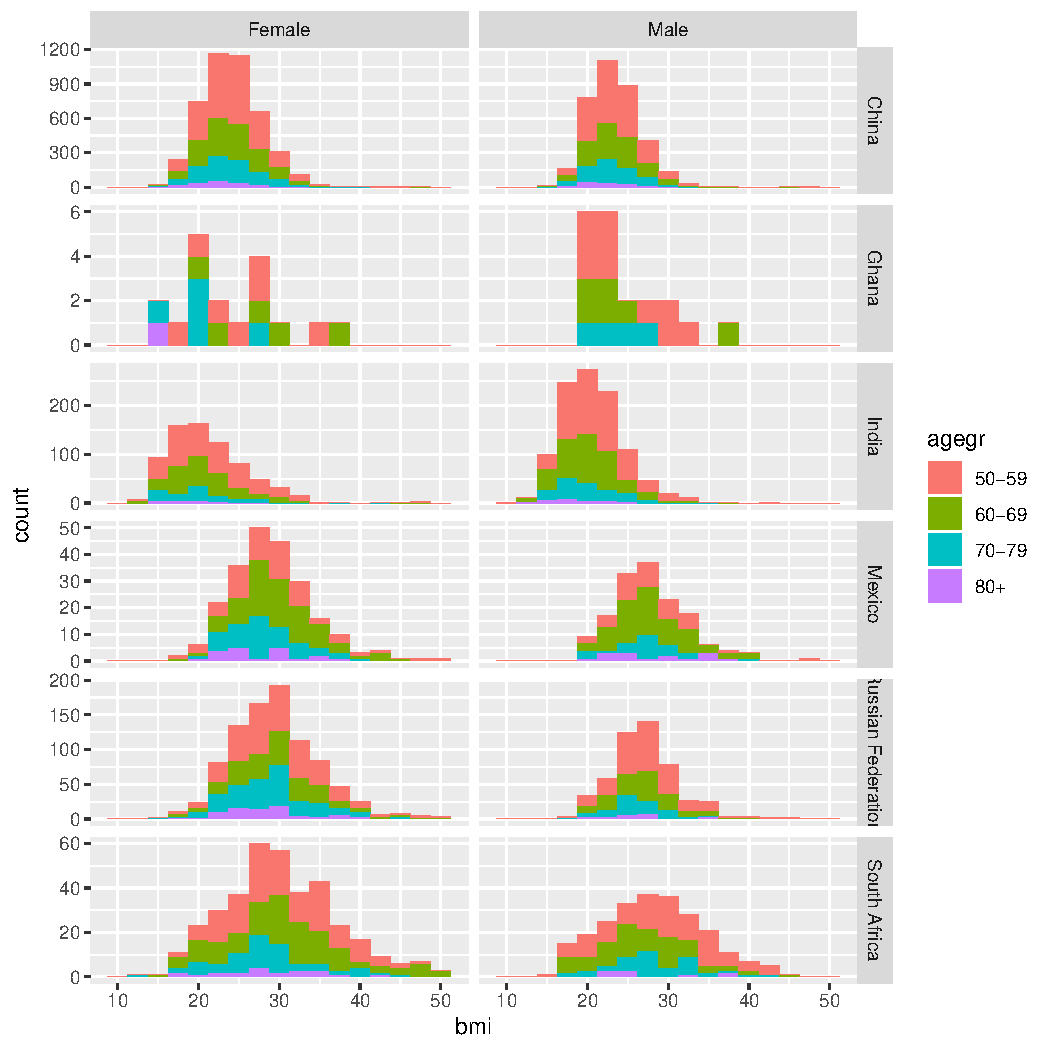
\includegraphics[width=\maxwidth]{figure/L1_FacetedHistograms-1} 

\end{knitrout}

Note the 'free' y-axis. Its not obvious at first glance that China has much more data than South Africa.  An annotation on the plot of the total numbers would draw immediate attention to this. Note too that Ghana's data set (after removal of the NA's) is \textsl{very} small. For some unexplained reason, the Ghana data has very few height measurements even though these are necessary for comutation of BMI.
Let's have a look at the data for disability vs age.

\begin{knitrout}
\definecolor{shadecolor}{rgb}{0.969, 0.969, 0.969}\color{fgcolor}\begin{kframe}
\begin{alltt}
 \hlstd{bP} \hlkwb{<-} \hlstd{bP} \hlopt \hlkwd{mutate}\hlstd{(}\hlkwc{bmi4} \hlstd{=} \hlkwd{factor}\hlstd{(bmi4,} \hlkwc{levels} \hlstd{=}
                                     \hlkwd{c}\hlstd{(}\hlstr{"Underweight"}\hlstd{,}\hlstr{"Normal"}\hlstd{,} \hlstr{"Pre-Obese"}\hlstd{,} \hlstr{"Obese"}\hlstd{)))}
\hlstd{p} \hlkwb{<-} \hlkwd{ggplot}\hlstd{(bP,} \hlkwd{aes}\hlstd{(}\hlkwc{x} \hlstd{= age,}  \hlkwc{y} \hlstd{= disability ,}\hlkwc{color} \hlstd{= residence,} \hlkwc{shape} \hlstd{= sex))} \hlopt{+}
  \hlkwd{geom_point}\hlstd{()} \hlopt{+}
  \hlkwd{facet_grid}\hlstd{(country}\hlopt{~}\hlstd{bmi4)}
\hlstd{p}
\end{alltt}
\end{kframe}
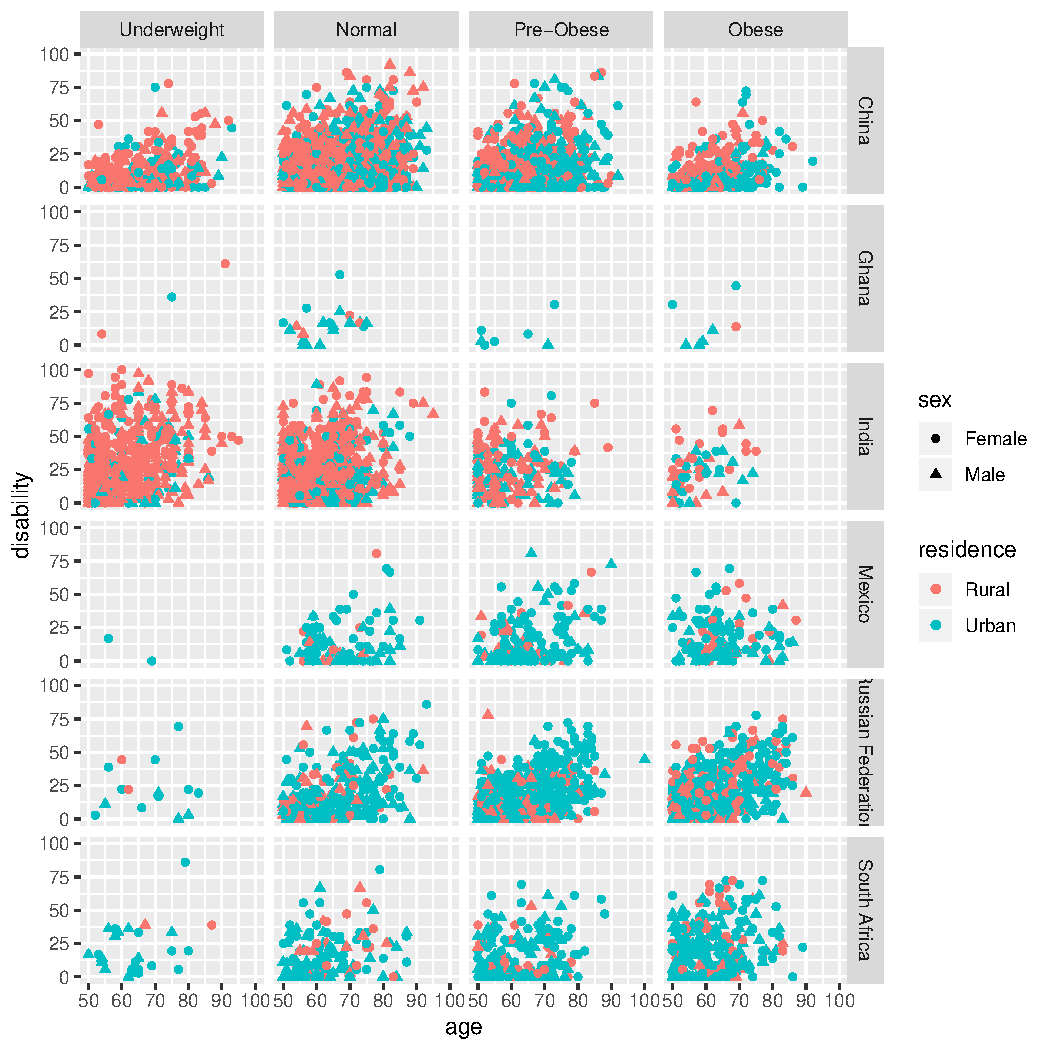
\includegraphics[width=\maxwidth]{figure/L1ScatterFacet-1} 

\end{knitrout}



%\printindex
\end{document}
